\begin{minipage}[b]{\textwidth}

\centering
\normalsize
\tikzset{every picture/.style={line width=0.75pt}} %set default line width to 0.75pt        

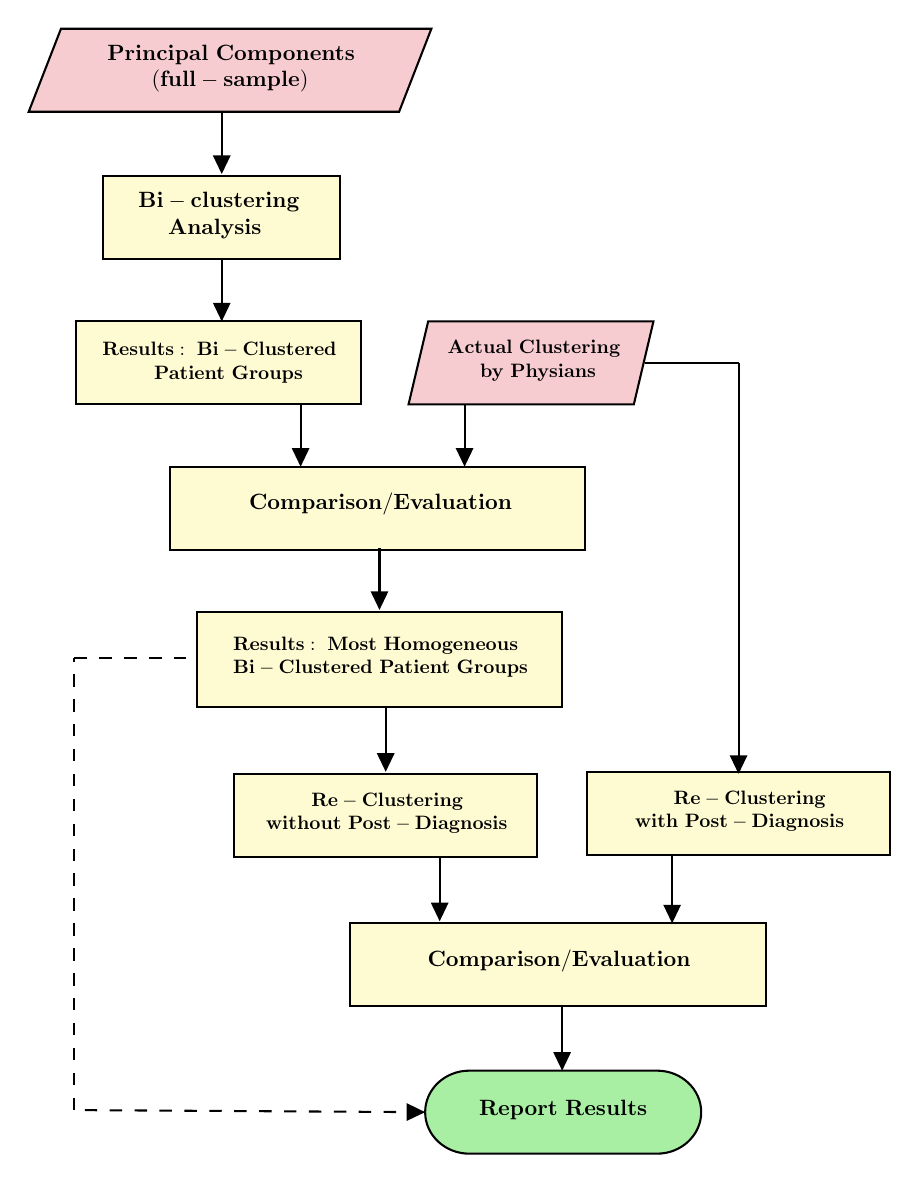
\begin{tikzpicture}[x=0.75pt,y=0.75pt,yscale=-1,xscale=1]
%uncomment if require: \path (0,606); %set diagram left start at 0, and has height of 606

%Shape: Parallelogram [id:dp6647145031150581] 
\draw  [fill={rgb, 255:red, 208; green, 2; blue, 27 }  ,fill opacity=0.2 ] (194.05,7) -- (372.5,7) -- (356.95,47) -- (178.5,47) -- cycle ;
%Straight Lines [id:da8846773602112543] 
\draw    (271.5,47) -- (271.5,75) ;
\draw [shift={(271.5,77)}, rotate = 270] [fill={rgb, 255:red, 0; green, 0; blue, 0 }  ][line width=0.75]  [draw opacity=0] (8.93,-4.29) -- (0,0) -- (8.93,4.29) -- cycle    ;

%Shape: Rectangle [id:dp27431555826277765] 
\draw  [fill={rgb, 255:red, 248; green, 231; blue, 28 }  ,fill opacity=0.2 ] (214.5,78) -- (328.5,78) -- (328.5,118) -- (214.5,118) -- cycle ;
%Straight Lines [id:da14961685906904876] 
\draw    (271.5,118) -- (271.5,146) ;
\draw [shift={(271.5,148)}, rotate = 270] [fill={rgb, 255:red, 0; green, 0; blue, 0 }  ][line width=0.75]  [draw opacity=0] (8.93,-4.29) -- (0,0) -- (8.93,4.29) -- cycle    ;

%Shape: Rectangle [id:dp09827610187608338] 
\draw  [fill={rgb, 255:red, 248; green, 231; blue, 28 }  ,fill opacity=0.2 ] (201.5,148) -- (338.5,148) -- (338.5,188) -- (201.5,188) -- cycle ;
%Straight Lines [id:da223473735957731] 
\draw    (309.5,188) -- (309.5,216) ;
\draw [shift={(309.5,218)}, rotate = 270] [fill={rgb, 255:red, 0; green, 0; blue, 0 }  ][line width=0.75]  [draw opacity=0] (8.93,-4.29) -- (0,0) -- (8.93,4.29) -- cycle    ;

%Straight Lines [id:da10156066919663931] 
\draw    (388.5,188) -- (388.5,216) ;
\draw [shift={(388.5,218)}, rotate = 270] [fill={rgb, 255:red, 0; green, 0; blue, 0 }  ][line width=0.75]  [draw opacity=0] (8.93,-4.29) -- (0,0) -- (8.93,4.29) -- cycle    ;

%Shape: Rectangle [id:dp1364397766049188] 
\draw  [fill={rgb, 255:red, 248; green, 231; blue, 28 }  ,fill opacity=0.2 ] (246.5,218) -- (446.5,218) -- (446.5,258) -- (246.5,258) -- cycle ;
%Straight Lines [id:da28849175814256767] 
\draw    (347.5,257) -- (347.5,285) ;
\draw [shift={(347.5,287)}, rotate = 270] [fill={rgb, 255:red, 0; green, 0; blue, 0 }  ][line width=0.75]  [draw opacity=0] (8.93,-4.29) -- (0,0) -- (8.93,4.29) -- cycle    ;

%Shape: Rectangle [id:dp855299838261038] 
\draw  [fill={rgb, 255:red, 248; green, 231; blue, 28 }  ,fill opacity=0.2 ] (259.5,288) -- (435.5,288) -- (435.5,334) -- (259.5,334) -- cycle ;
%Shape: Parallelogram [id:dp47004695097922267] 
\draw  [fill={rgb, 255:red, 208; green, 2; blue, 27 }  ,fill opacity=0.2 ] (370.96,148) -- (479.5,148) -- (470.04,188) -- (361.5,188) -- cycle ;
%Straight Lines [id:da06063407025060097] 
\draw    (475.5,168) -- (520.5,168) ;


%Straight Lines [id:da5926644195581223] 
\draw    (350.5,334) -- (350.5,363) ;
\draw [shift={(350.5,365)}, rotate = 270] [fill={rgb, 255:red, 0; green, 0; blue, 0 }  ][line width=0.75]  [draw opacity=0] (8.93,-4.29) -- (0,0) -- (8.93,4.29) -- cycle    ;

%Straight Lines [id:da8413098221287976] 
\draw    (520.5,168) -- (520.5,364) ;
\draw [shift={(520.5,366)}, rotate = 270] [fill={rgb, 255:red, 0; green, 0; blue, 0 }  ][line width=0.75]  [draw opacity=0] (8.93,-4.29) -- (0,0) -- (8.93,4.29) -- cycle    ;

%Shape: Rectangle [id:dp73563614757607] 
\draw  [fill={rgb, 255:red, 248; green, 231; blue, 28 }  ,fill opacity=0.2 ] (277.5,366) -- (423.5,366) -- (423.5,406) -- (277.5,406) -- cycle ;
%Shape: Rectangle [id:dp6744694293772151] 
\draw  [fill={rgb, 255:red, 248; green, 231; blue, 28 }  ,fill opacity=0.2 ] (333.5,438) -- (533.5,438) -- (533.5,478) -- (333.5,478) -- cycle ;
%Straight Lines [id:da43373610475282676] 
\draw    (376.5,406) -- (376.5,435) ;
\draw [shift={(376.5,437)}, rotate = 270] [fill={rgb, 255:red, 0; green, 0; blue, 0 }  ][line width=0.75]  [draw opacity=0] (8.93,-4.29) -- (0,0) -- (8.93,4.29) -- cycle    ;

%Straight Lines [id:da681049356627645] 
\draw    (488.5,405) -- (488.5,436) ;
\draw [shift={(488.5,438)}, rotate = 270] [fill={rgb, 255:red, 0; green, 0; blue, 0 }  ][line width=0.75]  [draw opacity=0] (8.93,-4.29) -- (0,0) -- (8.93,4.29) -- cycle    ;

%Straight Lines [id:da6627436883022095] 
\draw    (435.5,478) -- (435.5,507) ;
\draw [shift={(435.5,509)}, rotate = 270] [fill={rgb, 255:red, 0; green, 0; blue, 0 }  ][line width=0.75]  [draw opacity=0] (8.93,-4.29) -- (0,0) -- (8.93,4.29) -- cycle    ;

%Flowchart: Terminator [id:dp4539534632908053] 
\draw  [fill={rgb, 255:red, 139; green, 233; blue, 134 }  ,fill opacity=0.75 ] (390.78,509) -- (481.22,509) .. controls (492.97,509) and (502.5,517.95) .. (502.5,529) .. controls (502.5,540.05) and (492.97,549) .. (481.22,549) -- (390.78,549) .. controls (379.03,549) and (369.5,540.05) .. (369.5,529) .. controls (369.5,517.95) and (379.03,509) .. (390.78,509) -- cycle ;
%Straight Lines [id:da9928979089443342] 
\draw  [dash pattern={on 4.5pt off 4.5pt}]  (200.5,310) -- (259.5,310) ;


%Straight Lines [id:da9346137110249131] 
\draw  [dash pattern={on 4.5pt off 4.5pt}]  (200.5,528) -- (200.5,310) ;


%Straight Lines [id:da835721246834527] 
\draw  [dash pattern={on 4.5pt off 4.5pt}]  (367.5,528.99) -- (200.5,528) ;

\draw [shift={(369.5,529)}, rotate = 180.34] [fill={rgb, 255:red, 0; green, 0; blue, 0 }  ][line width=0.75]  [draw opacity=0] (8.93,-4.29) -- (0,0) -- (8.93,4.29) -- cycle    ;
%Shape: Rectangle [id:dp16102927554927304] 
\draw  [fill={rgb, 255:red, 248; green, 231; blue, 28 }  ,fill opacity=0.2 ] (447.5,365) -- (593.5,365) -- (593.5,405) -- (447.5,405) -- cycle ;

% Text Node
\draw (276,26) node [scale=0.8]  {$ \begin{array}{l}
\mathbf{Principal\ Components}\\
\ \ \ \ \ \ (\mathbf{full-sample})
\end{array}$};
% Text Node
\draw (272,97) node [scale=0.8]  {$ \begin{array}{l}
\mathbf{Bi-clustering\ }\\
\ \ \ \ \mathbf{Analysis}
\end{array}$};
% Text Node
\draw (272,168) node [scale=0.7]  {$ \begin{array}{l}
\mathbf{Results:\ Bi-Clustered\ }\\
\ \ \ \ \ \ \ \ \mathbf{Patient\ Groups}
\end{array}$};
% Text Node
\draw (422,167) node [scale=0.7]  {$ \begin{array}{l}
\mathbf{Actual\ Clustering}\\
\ \ \ \ \mathbf{\ by\ Physians}
\end{array}$};
% Text Node
\draw (348,236) node [scale=0.8]  {$\mathbf{Comparison/Evaluation}$};
% Text Node
\draw (348,310) node [scale=0.7]  {$ \begin{array}{l}
\mathbf{Results:\ Most\ Homogeneous}\\
\mathbf{Bi-Clustered\ Patient\ Groups}
\end{array}$};
% Text Node
\draw (351,385) node [scale=0.7]  {$ \begin{array}{l}
\ \ \ \ \ \ \ \mathbf{Re-Clustering\ }\\
\mathbf{without\ Post-Diagnosis}
\end{array}$};
% Text Node
\draw (434,456) node [scale=0.8]  {$\mathbf{Comparison/Evaluation}$};
% Text Node
\draw (436,528) node [scale=0.8]  {$\mathbf{Report\ Results}$};
% Text Node
\draw (521,384) node [scale=0.7]  {$ \begin{array}{l}
\ \ \ \ \ \ \mathbf{Re-Clustering\ }\\
\mathbf{with\ Post-Diagnosis}
\end{array}$};


\end{tikzpicture}

\end{minipage}